\chapter{Arabic Language and Machine Translation}
\pagestyle{fancy}\lhead{\textbf \footnotesize\it{Arabic Machine Translation}}
\pagestyle{fancy}\chead{} \pagestyle{fancy}\rhead{}
\pagestyle{fancy}\lfoot{\textbf {\small\it{Univ-Mascara/Computer Science: 2024}}} 
\pagestyle{fancy}\cfoot{} \pagestyle{fancy}\rfoot{\thepage}
%%%%%%%%%%%%%%%%%%%%%%%%%%%%%%%%%%%%%%%%
\section{Overview} \label{start2}
Translation has become difficult due to the intricate variations across languages \cite{dorr99}. For instance, certain words may have different meanings based on the context, or other words may not have equivalent translations in other languages. Additionally, translating idiomatic expressions calls for a thorough understanding of both the source and target languages. Further, structural variations like word order disparities between languages complicate translation.

Another difficulty is that a good translation needs to be faithful and fluent. A faithful translation accurately conveys the sense of the original text, whereas a fluent translation is easy to understand and sounds natural. A literal, faithful translation could result in an unpleasant and unnatural translation in the target language. For example, fluency rather than faithfulness is more critical when translating literary works. We might have to alter some of the meaning to keep the text flowing smoothly. Readers should feel as if it was written in their native language. The faithfulness of the translation, however, is prioritized when translating a technical manual or a legal document. Even if the translation is not fluent, it must be faithful and convey the same meaning. To produce accurate translations that balance faithfulness and fluency, human translators primarily rely on their experience, knowledge, and reasoning abilities. Due to these issues, various human translators will translate the same text in different ways.

Despite the complex linguistic distinctions, recent decades have seen significant improvements in machine translation. It is even applied in practical, real-world applications. For instance, we employ machine translation for cross-language information retrieval. It allows people to interact and obtain information in other languages.
Machine translation is also used to assist human translators. By creating a draft translation that human translators will edit, it expedites a time-consuming translation task (Plitt and Masselot, 2010). In addition, we can employ machine translation for translations that are speech- and image-centric. Speech-centric translation involves translating a text from a speech recognition system into another language before the text is fully formed. As a result, it mimics a live human interpretation.
Image-centric machine translation uses an optical character recognition system to translate the text included in images, such as billboard advertisements or street signs.

There are various methods for automating the challenging task of translation. Data-driven methods later supplanted the initial rule-based approaches. The most popular data-driven methods are Statistical Machine Translation (SMT) and Neural Machine Translation (NMT). Nevertheless, due to its remarkable successes, NMT has become state-of-the-art.

Language differences and the various machine translation approaches are briefly discussed in the sections that follow, Sections 2.2 and 2.2. Neural networks and NMT are explained in Sections 2.3 and 2.4. The evaluation of machine translation is covered in the final section, Section 2.5.

\section{Arabic Language}
Arabic is considered as one of the six official languages of the United Nation. It is the official language in 22 countries and spoken by more than 350 million people in 24 countries around the world \cite{almansor18}. The Arabic language is morphologically rich and complex, however, it is considered a low-resource language due to the lack of enough parallel dataset.

Arabic is well known for its complex morphology. It has different possibilities of word order that express the same sentence. According to word orders, Arabic sentences can be classified into 4 types: SVO\footnote{SVO: Subject-Verb-Object}, VSO, VOS and SOV \cite{alqudsi14}.

Translating the Arabic language into other languages engenders multiple linguistic problems, as no two languages can match, either in the meaning given to the conforming symbols or in the ways in which such symbols are arranged in sentences. Lexical, syntactic and semantic problems arise when translating the meaning of Arabic words into English and vice versa. Machine translation into morphologically rich languages (MRL) poses many challenges, from handling a complex and rich vocabulary that can reach hundreds of thousands or even millions, to designing adequate MT metrics that take morphology into consideration. 

Fehri\cite{fehri93}, Chalabi\cite{chalabi00} and Daimi\cite{daimi01} enumerated major issues involving Arabic in the following points:
\begin{itemize}
	\item Arabic is written from right to left.
	\item There are no capital letters in Arabic.
	\item Gender is used for all nouns (there are no neutral).
	\item Some letters have different shapes depending on their location within a word. e.g. The shape of letter (\RL{`}) in the start of a word is (\RL{`-}) like in \RL{`lb}, in the middle (\RL{-`-}) like in \RL{l`b} and at the end (\RL{`} or \RL{-`}) like in \RL{bl`} or \RL{wd`}.
	\item Arabic words can be partially, fully or not vocalized. Unvocalized words may generate ambiguities for MT. See Table~\ref{tab_voc}.
	\begin{table}[!htb]
		\centering
		\begin{tabular}{lll}
			\hline\\[-1.5ex]
			\multicolumn{1}{l}{Word} & \multicolumn{1}{l}{Transliteration} & \multicolumn{1}{l}{English meaning} \\[0.5ex]
			\hline\\[-1.5ex]
			\RL{`amara} & Eamara & build / live / was populated\\[0.5ex]
			\RL{`ammara} & Eam\~~ara & Live a long time\\[0.5ex]
			\RL{`omira} & Eomira & became populous\\[0.5ex]
			\RL{`ommira} & Eom\~~ira & Given a long life\\[0.5ex]
			\RL{`omaro} & Eumaru & Omar (noun) / plural of Umrah\\[0.5ex]
			\RL{`am"ro} & Eamoru & Age of\\[0.5ex]
			\RL{`om"ro} & Eumoru & Age of\\[0.5ex]
			\RL{`omoro} & Eumuru & Age of\\[0.5ex]
			\RL{`am"ruN} & EamorN & Age\\[0.5ex]
			\RL{`om"ruN} & EumorN & Age\\[0.5ex]
			\RL{`omoruN} & EumurN & Age\\[0.5ex]
			\RL{`amaruN} & EamarN & Head cover for women\\[0.5ex]
			\RL{`amarra} & Eamar\~~a & Strong tough man /\\[0.5ex]
			&  & Longest of everything /\\[0.5ex]
			&  & Shrewd malicious guy /\\[0.5ex]
			&  & Ferocious man\\[0.5ex]
			\hline
		\end{tabular}
		\caption{Possible meanings of the unvocalized Arabic word "\RL{`mr}" (Emr)}
		\label{tab_voc}
	\end{table}
	
	\item Arabic has a relatively free order of words. See Table~\ref{tab0}.
	\begin{table}[!htb]
		\centering
		\begin{tabular}{lll}
			\hline\\[-1.5ex]
			\multicolumn{1}{c}{Order} & \multicolumn{1}{c}{Sentence} & \multicolumn{1}{c}{English translation} \\[0.5ex]
			\hline\\[-1.5ex]
			VSO & \RL{^srba `mro almaA'a} & Drank Omar the water\\[0.3ex]
			OVS & \RL{almA'a ^srba `mro} & The water drank Omar\\[0.3ex]
			SVO & \RL{`mro ^srba almaA'a} & Omar Drank the water\\[0.5ex]
			VOS & \RL{^srba almaA'a `mro} & Drank the water Omar\\[0.5ex]
			\hline
		\end{tabular}
		\caption{Arabic free word order}
		\label{tab0}
	\end{table}
	
	\item Some Arabic vocalized words may have multiple senses (polysemy) depending on its context. See Table~\ref{tab_polysem}. 
	\begin{table}[!htb]
		\centering
		\begin{tabular}{lll}
			\hline\\[-1.5ex]
			\multicolumn{1}{l}{Word} & \multicolumn{1}{l}{Transliteration} & \multicolumn{1}{l}{English meanings} \\[0.5ex]
			\hline\\[-1.5ex]
			\RL{sA'il} & sA\}il & liquid, beggar, questioner \\[0.5ex]
			\RL{`ayn} & Eayn & eye, water source, gold \\[0.5ex]
			\hline
		\end{tabular}
		\caption{Examples of vocalized Arabic words polysemy}
		\label{tab_polysem}
	\end{table}
	
	\item The subject can be omitted. e.g. \RL{y^srb almaA'} (He drinks the water)
	\item Some words hold the meaning of a whole sentence. e.g. \RL{fa'AsqaynAkomUh} (and We gave it to you to drink).
	\item Copula verbs "to be" and "to have" do not exist in Arabic.
	\item The three letters root system can often engender ambiguous words.
	\item Feminine nouns are often derived from masculine nouns, e.g. \RL{mhnds} (Engineer male) \RL{mhndsT} (Engineer female). In some cases they are totally different, e.g. \RL{wld} (Boy) \RL{bnt} (Girl).
	\item In English the number system moves from singular to plural form directly, however Arabic language includes dual form by suffixing morpheme (\RL{An}) or (\RL{yn}) to the singular form. e.g. \RL{mhnds} (Engineer male) \RL{mhndsAn} or \RL{mhndsayn} (Two Engineers male).
	\item The plural form of Arabic masculine nouns is the result of suffixing morpheme (\RL{wn}) or (\RL{yn}) to the singular form.
	e.g. \RL{mhnds} (Engineer male) \RL{mhndsUn} or \RL{mhndsiyn} (Engineers male).
	\item  The plural form of Arabic feminine nouns is the result of suffixing morpheme (\RL{At}) to the singular nouns. e.g. \RL{mhndsT} (Engineer female) \RL{mhndsAt} (Engineers female). 
	\item Some words have no fixed rule for their plural form. e.g. \RL{.tbyb} (Doctor) \RL{'a.tibbaA'} (Doctors).
\end{itemize}
In addition to the preceding specific challenges to MT, common standard issues also are present in Arabic language, such as:
\begin{itemize}
	\item Multi word expressions (MWE) where the meaning of words collocation varies between partially to completely not derivable from its single constituents \cite{Kordoni14}. e.g. \RL{qA`dT `skryT}, (military base) is a phrase that is highly compositional. \RL{mdynT al-mlAhy}, (amusement park), lit. "city of amusements" is an expression that shows a degree of idiomaticity. In extreme cases the meaning of the expression as a whole is utterly unrelated to the component words, such as, \RL{frs Alnby}, (grasshopper), lit. "Horse of the Prophet".
	
	\item Idioms and idiomatic expressions are frequently used by Arabic speakers. They are a special challenge for MT systems, because their translation mainly does not outcome literally, but logically \cite{Zaninello20}. e.g. \RL{'a.zlam mn timsA.h} , lit. "More oppressive than a crocodile", has the idiomatic meaning of (crocodile tears).
	
	\item Named entities (NE) refer to abstract entities in the real world such as people (PER) such as \RL{al'amIr `bd-al-qAdr} (Emir Abdelkader), places (LOC) such as \RL{mkT} (Mecca), companies, and organizations that have an appropriate name (ORG) such as \RL{yAhU} (Yahoo). It also refers to expressions of date, time, space and quantity (MISC) such as \RL{sbtmbr} 8 (September 8th), \RL{dj}100 (100DZD) or \RL{k.g}25 (25Kgs).
	
	Due to the rich lexical variations and the absence of capitalization in Arabic, the task of named entities recognition (NER) is more difficult. Handling NE in Arabic MT is done very carefully based on :
	\begin{enumerate}
		\item meaning translation: e.g. \RL{al-'omam al-motta.hdaT} (The United Nations).
		\item phoneme transliteration: e.g. \RL{jUjl} (Google).
		\item mixture of meaning translation and phoneme transliteration: \RL{kArUlAynA al-^smAlyaT} (North Carolina), where "North" is translated and "Carolina" is transliterated.
	\end{enumerate}   
\end{itemize}

\section{Social Media}
Social media involves online spaces where individuals can post and share information with others. They have become crucial in contemporary communication, fundamentally reshaping how individuals connect, information disseminates, and communities form. These online environments, characterized by user-generated content and interactive features \cite{boyd08},  allow for the creation of virtual spaces fostering real-time interaction and knowledge sharing \cite{yaqub23}.

\textbf{Social Networking Sites (SNS):} Platforms like Facebook prioritize building and maintaining online social connections. Users can share personal updates, engage in discussions through comments and reactions, and participate in groups centered around shared interests \cite{segesten22}. Research suggests that SNS use can foster social capital by strengthening existing relationships and enabling the formation of new ones \cite{yoon14}.

\textbf{Media-Sharing Platforms:} Platforms like Instagram and YouTube focus heavily on the creation and dissemination of multimedia content. Users can share and discover photos, videos, and live streams, with features designed to enhance content visibility through hashtags and algorithmic recommendations \cite{rogers21}. Studies highlight the increasing influence of visual communication and the emergence of new social norms surrounding content creation and consumption on these platforms \cite{lu24}.

\textbf{Messaging Applications:} Platforms like WhatsApp and WeChat enable asynchronous and real-time communication between individuals and groups. These applications offer features like text messaging, voice calls, and video conferencing, facilitating private and semi-private communication, often replacing traditional communication methods \cite{lenhart15}. Research suggests that messaging applications can strengthen interpersonal bonds and serve as crucial tools for information sharing and community mobilization \cite{pang20}.

\textbf{Professional Networking Sites:} LinkedIn serves a distinct purpose within the social media landscape, focusing on professional networking and career development. Users create profiles highlighting their skills and experience, connect with colleagues and potential employers, and discover job opportunities \cite{ellison07}. Studies suggest that LinkedIn usage can positively impact career prospects by facilitating professional connections and knowledge exchange \cite{davis20}.

Social media platforms are a goldmine for data collection. 
However, in the case of Arabic, several issues arise due to the way language is used on these platforms. 
Users often tend to write in colloquial Arabic or a mix of colloquial Arabic and English characters (often referred to as Arabizi). 
This deviates from the standard Arabic used in formal writing. 
This informality poses challenges for data collection and analysis, as algorithms need to be able to understand these diverse and non-standard language patterns.
Another important aspect of Arabic language on social media is the use of dialects.
Arabic is a highly diverse language, with many different dialects and variations.
Users may choose to write in their local dialect, which can vary significantly from Modern Standard Arabic, the standardized form of the language.
With the spread of social media, new challenges arise to the Arabic MT such as:   
\begin{itemize}
	\item  \textbf{Non-standard speech}: which encompasses dialectal languages or the various colloquial forms of standard language. This text frequently contains slang, MWE and unreasonable abbreviations \cite{Moussallem19} like as "idk\footnote{I don’t know}" and "brb\footnote{Be right back}" in English or "hmd\footnote{\RL{al.hmd lillh} (Thank God)}" and "slm\footnote{\RL{salAm} (Peace)}" in Arabic. For best translation results, the MT system is required
	to identify such argot and try to map it to the target language.
	
	\item \textbf{Arabizi} (sometimes known as Arabic chat alphabet, Franco-Arabic, Arabish, Araby and	Mu’arrab): which is defined as writing informal Arabic dialects in Latin characters and Arabic numerals. This new style of writing doesn’t follow any type of rules, which leads to big variations in writing nearly all Arabic words. The following words present some examples of the Arabizi issue that machine translation systems have to solve \cite{Darwish15}:
	\begin{enumerate}
		\item The Modern Standard Arabic word \RL{t.hrIr}\footnote{Liberation} has the following popular Arabizi equivalents: ta7rir, tahrir, t7rir, t7reer, ta7reer, tahreer, etc.
		\item The dialectal spellings of the MSA words \RL{lA-yl`b}\footnote{He does not play} could be \RL{mAyl`b^s}, \RL{mAbyl`b^s}, \RL{myl`b^s}, \RL{myl`b^sI}, \RL{mAyl`b^sI} etc, and the resultant Arabizi could be: mayel3absh, mayel3abch, mabyelaabsh, mabyel3absh, mayel3abshi, mayel3abchi, etc.
	\end{enumerate}
\end{itemize}

\section{Natural Language Processing}
Natural Language Processing (NLP) is a branch of computer science dedicated to facilitating communication between computers and human languages. Its methodologies find application in social media for the analysis and comprehension of the extensive textual data produced by users (Huang, 2021). Below are several applications of NLP in social media:
\begin{enumerate}
	\item \textbf{Machine Translation:} NLP techniques are utilized to translate text from one language to another, facilitating cross-lingual communication and information access. Machine translation involves converting text from a source language into a target language while preserving meaning, context, and grammatical structure.

	\item \textbf{Text Classification:} NLP techniques involve categorizing text data into predefined categories or labels based on its content. This involves tasks such as sentiment analysis, spam detection, topic classification, and intent recognition in chatbots. Text classification is essential for organizing and analyzing large volumes of text data efficiently.
	
	\item \textbf{Named Entity Recognition (NER):} NLP algorithms aim to identify and extract named entities from unstructured text, such as names of people, organizations, locations, dates, numerical expressions, and other specific entities. NER is crucial for various applications, including information retrieval, entity linking, and knowledge graph construction.
	
	\item \textbf{Speech Recognition:} NLP algorithms transcribe spoken language into text, enabling voice-controlled applications, virtual assistants, and speech-to-text transcription services. Speech recognition involves converting audio signals into textual representations, which can then be further processed or analyzed.
	
	\item \textbf{Information Extraction:} NLP methodologies focus on extracting structured information from unstructured text sources, enabling the retrieval of specific data points or facts from documents, web pages, or other text-based sources. Information extraction techniques involve identifying relevant entities, relationships, and events mentioned in the text.
	
	\item \textbf{Text Generation:} NLP models are employed to generate human-like text based on given prompts or input. This includes tasks such as automated content creation, dialogue generation, language translation, and summarization. Text generation techniques leverage deep learning architectures such as recurrent neural networks (RNNs) and transformer models.
	
	\item \textbf{Document Summarization:} NLP techniques condense lengthy documents or articles into shorter summaries while preserving the main points and key information. Document summarization aims to provide a concise overview of the text, facilitating easier comprehension and information retrieval.
	
	\item \textbf{Question Answering:} NLP systems process natural language questions and retrieve relevant answers from large text corpora or knowledge bases. Question answering involves understanding the semantics and context of the question, searching for relevant information, and generating accurate responses.
	
	\item \textbf{Language Understanding:} NLP models aim to understand the semantics, context, and intent behind natural language expressions. Language understanding involves tasks such as text comprehension, semantic analysis, and context modeling, enabling machines to interpret human communication more effectively.

	\item \textbf{Dialog Systems:} NLP-powered conversational agents interact with users in natural language, providing assistance, answering queries, and engaging in dialogue across various domains. Dialog systems leverage techniques such as natural language understanding (NLU) and natural language generation (NLG) to enable seamless communication between humans and machines.
\end{enumerate}
Natural Language Processing (NLP) emerges as a transformative force, enriching our lives by bridging the gap between human language and computing systems. This remarkable technology enables machines to comprehend, interpret, and generate human language, revolutionizing how we interact with technology. Through NLP, machines can analyze vast volumes of textual data from diverse sources such as social media, news articles, and customer reviews, extracting meaningful insights that shape various aspects of our lives. From facilitating accurate language translation and sentiment analysis to powering virtual assistants and chatbots, NLP permeates numerous applications, enhancing efficiency and convenience in our daily activities. Its significance lies in its ability to decipher the intricacies of human communication, empowering individuals and businesses alike with deeper understanding and actionable intelligence.

\section{Machine Translation}
Machine Translation is a procedure that uses computer pieces of software to express text from one natural language NL (SL i.e. source language) in another NL (TL i.e. target language). In any human or automated translation process, the meaning of the source sentences must be fully reproduced into the target translated sentences, which is only simple on the surface.

\begin{figure}[htbp]
	\centerline{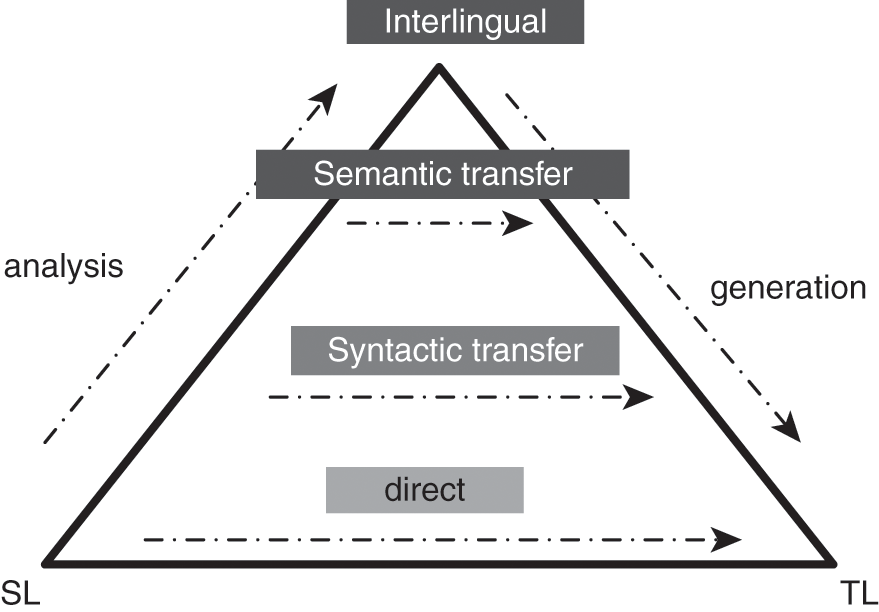
\includegraphics[scale=.7]{Figures/fig1.4.png}}
	\caption{The Vauquois triangle, illustrating the foundations of machine translation.}
	\label{fig1.4.png}
\end{figure}

The different approaches to MT fall into three categories: methods that depend on rules and knowledge (linguistic-based). Approaches that are empirical and data-driven (corpus-based); and finally, hybrid methods.

\subsection{Linguistic Approaches}
These MT approaches attempt to formalize all the necessary knowledge required for translation, using expert methods. The "Vauquois triangle" presented in Figure~\ref{fig1.4.png} is a generic representation of these techniques.

\subsubsection{\textbf{Direct Approach}}
or Direct MT (DMT) is, the simplest MT approach. It operates at the word level, i.e. the words' translation is done word by word, just, as a dictionary does, and generally without much correspondence of their meaning \cite{okpor14}.

\subsubsection{\textbf{Rule-based MT}}
(RBMT) uses linguistic knowledge of source and target languages fundamentally collected from (bilingual) dictionaries and grammars encompassing the principal morphological, syntactic and/or semantic rules of each language
respectively \cite{okpor14}. 
RBMT approach suffers from the impossibility of writing all the rules of all the languages, because this task requires large and important linguistic knowledge. %\cite{Charoenpornsawat02}.

\subsubsection{\textbf{Interlingual MT}}
The term "Interlingua" refers to a language that serves as a bridge between two languages. In this method, SL is turned into an assistant/mediator language (representation) which is independent of the languages concerned by the translation. This auxiliary form is then used to specify the TL's translated verse. This approach focuses on a single representation for different languages \cite{Ashraf15}.

\subsubsection{\textbf{Transfer-based MT}}
(TBMT) is similar to Interlingual-MT in that it generates a translation from an intermediate structure that mimics the original sentence's meaning. The source text is translated into a less language-specific intermediate representation. This form is then translated into a target language structure with a comparable structure, and the text is generated in the target language. The source and target languages' morphological, syntactic, and/or semantic information is used in the transfer process. As a result, TBMT can make use of knowledge of both the source and target languages. \cite{DO11}. 

\subsection{Corpus Approaches}
Corpus techniques use empirical methods to ensure that all linguistic knowledge is learned empirically and automatically from corpora, which are collections of parallel datasets of source and target phrases that are translated to each other.

\subsubsection{\textbf{Example-based MT}}
The main idea behind (EBMT) is analogy \cite{Nagao84}. The primary concept is to build new translations on top of current examples. Bilingual parallel corpora containing sentence pairs are used to train EBMT systems. It's used to translate similar-sounding sentences by looking for the closest source example to the source word or phrase in parallel corpora. Nagao has appropriately classified this procedure into three steps \cite{Nagao84}:
\begin{itemize}
	\item Fragments are matched against a database of real examples.
	\item Identifying the translation fragments that correlate (Alignment)
	\item Putting these together to create the target text
\end{itemize}

\subsubsection{\textbf{Statistical MT}}
(SMT) generates translation hypotheses in a target language $t$ based on a sentence in a source language $s$ with the highest conditional probability $P(t|s)$ \cite{brown88,brown93}. The translation direction will be inverted to a translation model (TM) $P(s|t)$ and a language model (LM) $P(t)$ will be included by applying the Bayes rule. The following equation~\eqref{eq:eq1} is used to optimize the likelihood of the best translation:
\begin{equation}
	\label{eq:eq1}
	t_{best}=arg_{t}max(P(t|s))=arg_{t}max(P(s|t) \times P(t))
\end{equation}
where $P(s|t)$ is the TM and $P(t)$ is the LM.

\begin{figure}[htbp]
	\centerline{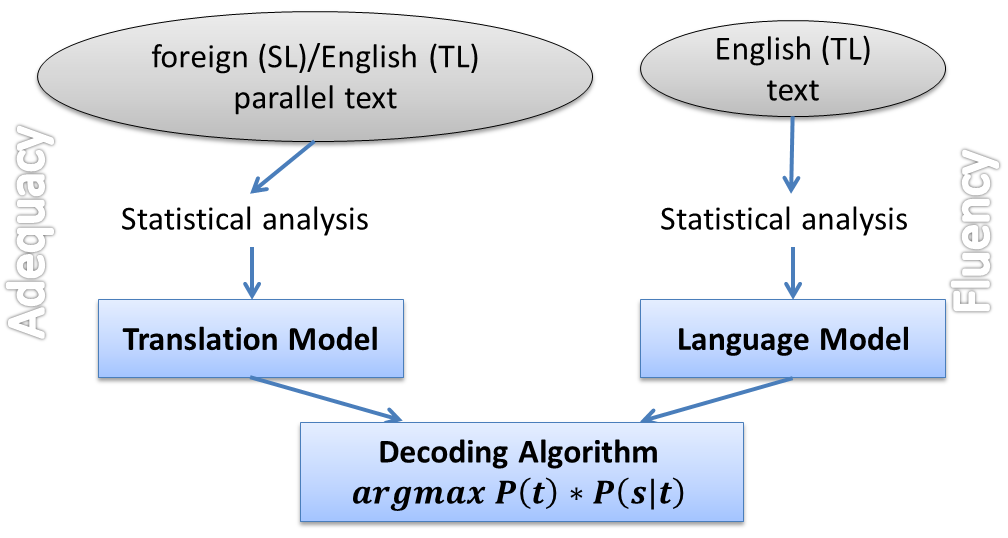
\includegraphics[scale=0.3]{Figures/fig1.13.png}}
	\caption{Statistical Machine Translation approach}
	\label{fig1.13.png}
\end{figure}

SMT requires a language model, a translation model, and a decoding method in general. The TM, on the one hand, assures that the target hypothesis created matches the source sentence. The LM, on the other hand, ensures that the output is grammatically correct  (Figure~\ref{fig1.13.png}).

\section{Evaluation}
As an integral part of design science research, evaluation is crucial to assessing the quality of machine translation outputs and comparing different machine translation methods. We need to measure quality to track progress, ideally with a single score.
However, devising such a score is still an open research question (Koehn, 2020).
Nonetheless, some best practices have already been established, and in general,
there is broad consensus on how to track quality gains.
Human (Section 2.5.1) and automatic (Section 2.5.2) evaluation methods exist.
Human evaluation seems more accurate than automatic evaluation because the
translation is, after all, intended for humans. However, running a human evaluation can be time-consuming and expensive.
In practice, it can be used to compare a small number of variant systems. Therefore, automated metrics are prevalent because they can rapidly evaluate system improvements; they are also used as a loss function for training models.

\subsection{Human Evaluation}
Human evaluation can be considered the most common method of judging and measuring translation quality. The linguistics and translation experts can judge the quality of a translation system output from two corners: 
\begin{itemize}
	\item \textbf{Fluency}: The level of smoothness and coherence of the translated text to target language norms,  such as grammaticality, intelligibility and clarity.  When annotating fluency, the evaluators (fluent only in the target language) have access to only the translation being evaluated and not the source text which is not relevant to the fluency assesment. 
	\item \textbf{Adequacy}: Also known as accuracy. It stands for the correspondence of the target text to the source text, including the expressive means in translation, and how well the target text represents the informational content of the source text. In this case, the bilingual evaluators (in both the source and target languages) have access to the source text and translations being evaluated and habitually, they take into consideration the context of the sentence.   
\end{itemize}
The fluency and adequacy are usually measured on a 5-point scale, as presented in the following table \ref{tab:table1.1} \cite{mauvcec19}.

\begin{table}[ht]% <--- it say "let figure be here"
	\centering
	\resizebox{\textwidth}{!}{%
		\begin{tabular}{@{}lccccc@{}}
			\toprule
			\multirow{2}{*}{\textbf{Adequacy}} & \textbf{1}           & \textbf{2}           & \textbf{3}           & \textbf{4}           & \textbf{5}           \\ \cmidrule(l){2-6} 
			& None                 & Little meaning       & Much meaning         & Most meaning         & All meaning          \\ \midrule
			& \multicolumn{1}{l}{} & \multicolumn{1}{l}{} & \multicolumn{1}{l}{} & \multicolumn{1}{l}{} & \multicolumn{1}{l}{} \\ \midrule
			\multirow{2}{*}{\textbf{Fluency}}  & \textbf{1}           & \textbf{2}           & \textbf{3}           & \textbf{4}           & \textbf{5}           \\ \cmidrule(l){2-6} 
			& Incomprehensible     & Disfluent language   & Non-native language  & Good language        & Flawless language    \\ \bottomrule
		\end{tabular}%
	}
	\caption{Numeric scale for adequacy and fluency evaluation.}
	\label{tab:table1.1}
\end{table}

Human evaluation is intrinsically subjective and expensive in time and money. To reduce the problem of subjectivity, more experts are usually invited to evaluate the same translations in the ES, and their assessments are, eventually, justified statistically.

\subsection{Automatic Evaluation} 
Generally, translation evaluation methods are based on counting word- and/or sentence-based errors likely to be identified automatically.
Correlation with human evaluation is the measure of evaluation for metrics.
Different metrics are used in MT evaluation: BLEU \cite{papineni02}, NIST \cite{doddington02}, METEOR \cite{banerjee05}, TER \cite{snover06}, LEPOR \cite{han12} and many others. 
All of these metrics require reference translations because they confront the MT output sentences with reference translations and produce comparison scores.\\
\textbf{BLEU} metric is one of the first and most used metrics to return high correlation with human evaluation of quality. 
It measures the overlap of single words (unigrams) and \textit{n}-grams between MT output and reference translations. 
BLEU operates by not only counting matching words between the translation and reference but also accounting for n-gram alignments. 
This approach values proper word sequencing, enhancing the chances of aligning word pairs (bigrams) or longer sequences like trigrams or 4-grams. 
Additionally, multiple reference translations can be employed to assess the presence of $n$-gram matches across variations.
The BLEU score of a machine-translated output relies on the adjusted $n$-gram precision along with a brevity penalty. 
Essentially, precision measures the proportion of $n$-grams in the machine translation output that align with the reference translation.
BLEU scores are calculated across an entire test set, typically with one or more reference translations. 
However, it's uncommon in practice to utilize multiple reference translations.
\begin{equation}
	BLEU = BP * exp \sum_{n=1}^N log \frac{matching\_i\_grams}{total\_i\_grams}
%	BLEU=BP*\left(\sum_{n=1}^N w_n log\left(precision_n\right)\right)
	\label{eqn:BLEU}
\end{equation}
The brevity penalty (BP) in Equation \ref{eqn:BLEU}, which penalizes shorter output, is expressed as:
\begin{equation*}
	BP = min(1,\frac{output\_length}{reference\_length}).
\end{equation*}
%\[
%BP=\begin{cases} 
%	1 & if c > r\\ 
%	e^{(1-r/c)} & if c \leq r
%\end{cases}
%\]
\\BLEU suffers from notable drawbacks, one of which is its stringent nature. 
For instance, it incorporates trigram or 4-gram precision in its calculation. 
However, a translated sentence might lack any trigram or 4-gram matches with the reference translation, leading to a BLEU score of zero.
\section{Related Work}
The main focus of AMT (Arabic Machine Translation) research initially was on translating from Modern Standard Arabic (MSA) to English, with significantly less emphasis on the reverse direction, from English to Arabic, and even fewer efforts dedicated to translations between Arabic and other languages. 
The first direct-based machine translation system from English to Arabic was developed by Weidner Communication Inc. In 1990, Apptek introduced ArabTrans MT, a tool for translating from English to Arabic. 
Additionally, products like Al-Mutarjim Al-Araby, Al-Alamiyah, and Al-Nakheel were capable of translating between French and Arabic as well as English and Arabic. 
A critical challenge in using the Interlingua approach for AMT is the construction of representations that resolve ambiguity and accurately reflect the semantic structure of the language. 
There have been limited studies that have developed and assessed models using this method.
Table~\ref{tab_linguistic} summarizes the surveyed AMT research studies.
\begin{small}
	\begin{longtable}{|l|l|l|l|l|}
		\hline
		Year & Research & SL-TL$^{\mathrm{a}}$ & Method & Score\\
		\hline
		\endhead
		%	\hline
		%	\endfoot
		
		\multicolumn{5}{c}{\textbf{\textcolor{blue}{Linguistic-based AMT researches}}}\\
		%	\hline
		\multicolumn{5}{l}{\textbf{Direct-based AMT}}\\
		\hline
		2005 & Al-Taani \& Hailat \cite{altaani05}					& En$\rightarrow$Ar &-& 57.3\%\\
		2007 & Ittycheriah \& Roukos \cite{ittycheriah-roukos-07}	& Ar$\rightarrow$En &Word alignment& Bl 51.27\\
		\hline
		\multicolumn{5}{l}{\textbf{Rule-based AMT}}\\
		\hline
		1995 & Mankai \& Mili \cite{mankai95}				& Ar$\rightarrow$En/Fr &-&\\
		2008 & Salem et al. \cite{salem08} 					& Ar$\rightarrow$En &-&\\
		2008 & Nguyen \& Vogel \cite{nguyen08}				& Ar$\rightarrow$En &-& 56.03\\
		2008 & Samy	\& & Ar-Sp-En &-&\\
		 & Gonz{\'a}lez-Ledesma \cite{samy08}	&  &-&\\
		2008 & AbuShuqier \& Sembok \cite{abushquier08} 	& En$\rightarrow$Ar &-& 96.1\%\\
		2009 & Elming \& Habash \cite{elming09}				& En$\rightarrow$Ar &-&\\
		2009 & Besançon et al. \cite{besanccon09} 			& En/Fr$\rightarrow$Ar &-&\\
		2012 & Salloum \& Habash \cite{salloum12}			& DA$\rightarrow$MSA &-&\\
		2020 & Sghaier \& Zrigui \cite{sghaier20}			& DA$\rightarrow$MSA &-& Bl 55.22\\
		\hline
		\multicolumn{5}{l}{\textbf{Interlingua-based AMT}}\\
		\hline
		2002 & Soudi et al. \cite{soudi02}					& En$\rightarrow$Ar &-&\\
		2006 & Shaalan et al. \cite{shaalan06}				& En$\rightarrow$Ar &-&\\
		2008 & Bouillon et al. \cite{bouillon08}			& Jp$\leftrightarrow$Ar &-&\\
		2014 & Al Ansary \cite{AlAnsary14}					& En$\rightarrow$Ar &Universal Networking Language&\\
		\hline
		\multicolumn{5}{l}{\textbf{Transfer-based AMT}}\\
		\hline
		2002 & Attia \cite{attia02}							& En$\rightarrow$Ar &Agreement features&\\
		2004 & Shaalan et al. \cite{shaalan04}				& En$\rightarrow$Ar &-& 92\%\\
		2010 & Shirko et al. \cite{shirko10}				& Ar$\rightarrow$En &-& 94.6\%\\
		2010 & Shaalan et al. \cite{shaalan10a}				& En$\leftrightarrow$Ar &-& 0.450%4
		/0.458%1
		\\
		2011 & Hatem et al. \cite{hatem11}					& En$\rightarrow$Ar &Morphological analysis&\\
		\hline
		\multicolumn{5}{c}{\textbf{\textcolor{blue}{Corpus-based AMT researches}}}\\
		%	\hline
		\multicolumn{5}{l}{\textbf{Example-based AMT}}\\
		\hline
		2002 & Guidere \cite{guidere02}					& Fr-Ar &-&\\
		2011 & Bar \& Dershowitz \cite{Bar11}			& Ar$\rightarrow$En &Verb paraphrases& 23.98\\
		2012 & Bar \& Dershowitz \cite{Bar12}			& Ar$\rightarrow$En &Semantic equivalents&\\
		2012 & Cavalli-Sforza \& Phillips \cite{Cavalli-Sforza12}	& Ar$\rightarrow$En &Morphological analysis&\\
		2014 & El-Shishtawy 		& En$\rightarrow$Ar &Template-based syntactic &\\
		&\& El-Sammak \cite{elshishtawy14}		& & matching&\\
		\hline
		\multicolumn{5}{l}{\textbf{Statistical-based AMT}}\\
		\hline
		2006 & Hasan et al. \cite{hasan06}				& Ar$\rightarrow$Fr &Pre-/Post-processing& 40.8\%\\
		2007 & Diab et al. \cite{diab07}				& Ar$\rightarrow$En &Pre-/Post-processing& 45.38\%\\
		2007 & Sarikaya \& Deng \cite{sarikaya07}		& En$\rightarrow$Ar &POS tag$^{\mathrm{b}}$/CDW$^{\mathrm{d}}$&+0.3\\
		2009 & Badr et al. \cite{badr09}				& En$\rightarrow$Ar &Syntactic phrase reordering&Bl 32.46\\
		%s		2009 & Mostefa et al. \cite{mostefa09}					& Ar-Fr-En\\[0.3ex]
		2009 & Habash \& Hu \cite{habash-hu09}		& Ar$\rightarrow$En$\rightarrow$Cn &MT Evaluation&Bl +1.1\\
		2010 & Carpuat et al. \cite{carpuat10}			& Ar$\rightarrow$En &Word reordering&Bl 51.70\\
		2010 & Ghurab et al. \cite{ghurab10}			& Ar$\leftrightarrow$Cn &-&0.805%3
		/0.696%5
		\\
		2010 & Bisazza and Federico \cite{bisazza10}	& Ar$\rightarrow$En &Word reordering& 48.96\\
		2017 & Durrani et al. \cite{durrani17}			& Ar$\leftrightarrow$En &MT Evaluation& Bl +4\\	
		2017 & Mallek et al. \cite{mallek17}			& Ar$\leftrightarrow$En &Pre- processing& Bl 10.98\\
		2017 & Ebrahim et al. \cite{ebrahim17}			& En$\rightarrow$Ar &MWE Detection& 19.31/19.22\\
		2019 & Aqlan et al. \cite{aqlan19a}				& Ar$\rightarrow$Cn &Morpho/Vocab/POS tag& Bl 19.40\\
		\hline
		\multicolumn{5}{c}{\textbf{\textcolor{blue}{Hybrid AMT}}}\\
		\hline
		2004 & Alsharaf et al. \cite{alsharaf04}	& Fr$\rightarrow$Ar& Direct+Transfer+Pivot+SMT &\\
		2008 & Toutanova et al. \cite{toutanova08}	& En$\rightarrow$Ar& Inflection prediction models &Bl 36.92\\
	 & 	& &  + SMT &\\
		2008 & Hatem \& Nassar \cite{hatem08}		& En$\rightarrow$Ar& Rule-based + Example-based & 68\%\\
		2009 & Matusov et al. \cite{matusov09} 		& Ar$\rightarrow$En& Multi-engine (5 MT systems) &\\
		2009 & Habash et al. \cite{habash09}		& Ar$\rightarrow$En& SMT + Rule-based &Bl 0.4162\\
		2010 & Al Dam \& Guessoum \cite{aldam10}   	& En$\rightarrow$Ar& Transfer-based + ANN &56\%\\
		2010 & Sawaf \cite{sawaf10}					& DA$\rightarrow$MSA& Rule-based+SMT & 42.1\%\\
		2011 & Alawneh \& Sembok \cite{alawneh11}	& En$\rightarrow$Ar& Rule-based + Example-based &\\
		2012 & Shaalan \& Hany \cite{shaalan12}		& Ar$\rightarrow$En& Rule-based + Example-based & WER 88\%\\
		2014 & Akeel \& Mishra \cite{akeel14}   	& En$\rightarrow$Ar& Rule-based + ANN & 0.6\\
		2015 & Mohamed \& Sadat	\cite{mohamed15}	& Ar$\rightarrow$Fr& Morphological rule + SMT & 34.7\%\\
		2015 & Zantout \& Guessoum \cite{zantout15}	& Ar$\rightarrow$En& Transfer-based + ANN &64.50\%\\
		\hline
		\multicolumn{3}{l}{$^{\mathrm{a}}$Source language-Target language}&
		\multicolumn{2}{l}{$^{\mathrm{b}}$Part Of Speech Tagging}\\
		\multicolumn{3}{l}{$^{\mathrm{c}}$Context Dependent Words}\\
		\caption{Linguistic-, Corpus-based and Hybrid AMT researches}
		\label{tab_linguistic}\\
	\end{longtable}
\end{small}

\section{Summary}
In conclusion, this chapter has delved into the multifaceted challenges and intricacies surrounding Arabic language processing, with a specific focus on machine translation (MT).
We have explored the intricate aspects of Arabic, ranging from its morphology and syntax to its diverse array of dialects, all of which present formidable hurdles for natural language processing (NLP) and MT systems alike. 
Additionally, we have scrutinized the influence of social media on Arabic NLP and MT, taking into account the unique linguistic characteristics and informal language usage prevalent on online platforms. 
 
Our examination has encompassed both linguistic and corpus-based approaches to Arabic MT, underscoring the necessity of tailored resources and datasets to capture the language's nuances effectively. 
Moreover, we have delved into various MT evaluation methods, encompassing both human and automatic assessment techniques. 
 
Lastly, we have surveyed the related work in the field, providing insights into recent advancements, methodologies, and the challenges encountered in Arabic language MT research, thus offering valuable perspectives on the current landscape and future trajectories of the field.